%!TEX root = ../main.tex

\chapter{Theoretische Grundlagen}

\section{Aufbau und Alterungsmechanismen von \acs{LIB}}
Elektrofahrzeuge nutzen überwiegend \acs{LIB}, die sich aus zahlreichen Zylinder- oder Pouch-Zellen zusammensetzen. Abbildung \ref{fig:pouch-zylinder-zelle} zeigt beispielhaft beide Zellformate. 
\begin{figure}[H]
	\centering
	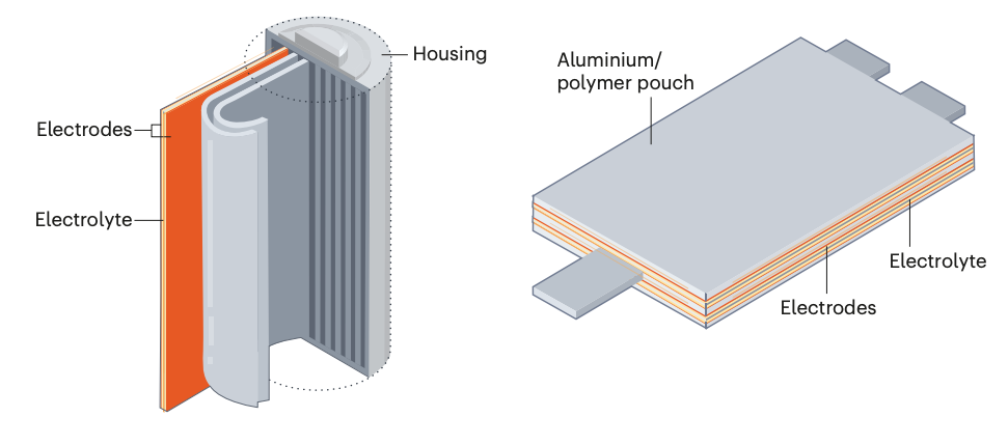
\includegraphics[height=0.25\linewidth]{resources/images/pouch-zylinder-zelle}
	\caption{Beispiel einer Zylinder- (links) und einer Pouchzelle (rechts)}
	\label{fig:pouch-zylinder-zelle}
\end{figure}

Zylinderzellen zeichnen sich durch eine hohe mechanische Stabilität und einer langen Lebensdauer aus, erfordern jedoch eine aufwendigere Kühlung und weisen bei gleichem Bauvolumen eine geringere Energiedichte als Pouch-Zellen auf. Zugleich ermöglichen Pouch-Zellen flexible Bauformen und höhere Energiedichten, neigen jedoch während des Alterungsprozesses zur Volumenexpansion (Swelling), was die Batteriealterung beschleunigt \cite{articlePouchZellenAlterung}.
\\
Unabhängig vom Zellformat besteht eine \acs{LIB} aus Anode, Kathode, Separator, Stromkollektoren und Elektrolyt \cite{urlIdRecentAdvancementsLIB}, wie in Abbildung \ref{fig:aufbau-nmc-zelle} dargestellt. Diese Komponenten ermöglichen einen Ionenfluss im Zellinnern und einen gleichzeitigen Elektronenfluss im äußeren Stromkreis, damit elektrischer Strom fließen kann \cite{urlIdLIBFUnktionsweise}.
\begin{figure}[H]
	\centering
	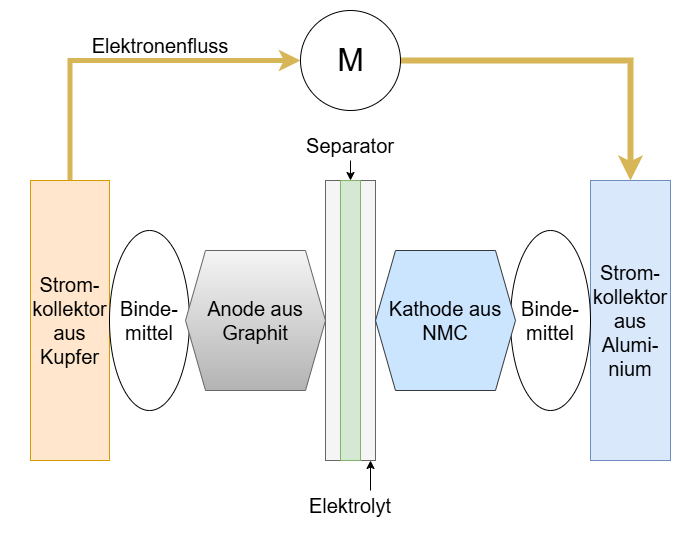
\includegraphics[height=0.4\linewidth]{resources/images/aufbau-nmc-zelle}
	\caption{Aufbau einer \acs{LIB}-Zelle beim Entladeprozess \cite{articleAlterungLithiumBatterien}}
	\label{fig:aufbau-nmc-zelle}
\end{figure}

Beim Entladen einer \acs{LIB} oxidiert Lithium in der Graphitanode unter Freisetzung von \ce{Li+}-Ionen und Elektronen. Diese Elektronen fließen über den Kupfer-Stromkollektor durch den äußeren Stromkreis zum Aluminium-Stromkollektor und treiben dabei elektrische Verbraucher an. Parallel dazu diffundieren die \ce{Li+}-Ionen durch das Elektrolyt und den Separator zur Kathode aus \ac{NMC}, wo sie in die Kristallstruktur eingelagert werden \cite{urlIdLIBFUnktionsweise}. Im Ladeprozess laufen die elektrochemischen Reaktionen umgekehrt ab. Lithium wird an der NMC-Anode oxidiert, wobei Elektronen über den Aluminium-Stromkollektor und den äußeren Stromkreis zum Kupfer-Stromkollektor fließen. Die \ce{Li+}-Ionen wandern erneut durch das Elektrolyt, passieren den Separator und lagern sich in der Graphitkathode ein \cite{urlIdLIBFUnktionsweise}.
\\
Somit sind Kathode und Anode jeweils für die Interkalation bzw. Deinterkalation von \ce{Li+}-Ionen sowie für die zugehörigen Redoxreaktionen (Reduktion bzw. Oxidation) verantwortlich. Die Stromkollektoren sorgen für eine leitfähige Verbindung zwischen Elektrodenmaterial und äußerem Stromkreis, sodass Elektronen effizient abgeleitet werden. Der Separator verhindert einen Kurzschluss, in dem er Ionen, aber keine Elektronen passieren lässt und so den direkten Kontakt der Elektroden unterbindet. Zuletzt ermöglicht das Elektrolyt den \ce{Li+}-Ionen-Transport zwischen Kathode und Anode \cite{urlIdDifferentAgingMethodsForLIBs}.
\\
Um den aktuellen Zustand einer \acs{LIB} zu bewerten, werden die Kenngrößen \ac{SoC}, \ac{SoH}, Kapazität und Innenwiderstand herangezogen. Der \acs{SoC} beschreibt den aktuellen Ladezustand relativ zur Gesamtkapazität und wird üblicherweise in Prozent angegeben. Der \acs{SoH} informiert über den Gesundheitszustand der Batterie, in dem er das Verhältnis zwischen aktuell verfügbarer Kapazität zur ursprünglichen Nennkapazität darstellt \cite{urlIdSoCSoHDependencyLIBs}. Die Kapazität selbst, typischerweise in Amperestunden (Ah) angegeben, definiert die maximal speicherbare elektrische Ladung einer Batterie und nimmt mit zunehmender Alterung kontinuierlich ab \cite{articleAlterungLithiumBatterien}. Ein erhöhter Innenwiderstand führt zu Spannungsabfällen unter Last sowie einer verstärkten Wärmeentwicklung und wirkt sich somit negativ auf die Leistungsfähigkeit und Lebensdauer der Batterie aus \cite{urlIdBatterieALterungInternerWiderstand}.
\\
Die Alterung von Batterien lässt sich in kalendarische und zyklische Alterung unterteilen. Erstere tritt unabhängig von Lade- und Entladezyklen auf, während letztere durch Lade- und Entladevorgänge bedingt wird. Beide Alterungsformen werden durch interne Faktoren, wie \ac{SEI} \cite{urlIdBatterieAlterungSEI}, \ac{CEI} \cite{urlIdBatterieAlterungCEI} und Lithium-Plating \cite{urlIdBatterieAlterungLithiumPlating}, sowie externen Faktoren, wie \acs{SoC} \cite{urlIdBatterieAlterungVerschiedenerSoCLithiumBatterien}, \ac{DOD} \cite{urlIdAlterungDOD}, C-Rate \cite{urlIdBatterieNiedrigeTemperaturenLithiumBatterien} und Temperatur \cite{urlIdBatterieAlterungTemperatur}, \cite{urlIdBatterieAlterungTemperatur2}, beeinflusst.
\\
\acs{SEI} ist eine Grenzschicht, die sich bei den ersten Ladezyklen an der Grenzfläche zwischen Graphitanode und Elektrolyt bildet. Dabei binden sich \ce{Li+}-Ionen irreversibel ein und stehen nicht mehr dem elektrochemischen Prozess zur Verfügung. Während des Alterungsprozesses verdickt sich diese Schicht, wodurch die \ce{Li+}-Ionen-Konzentration kontinuierlich sinkt. Als Folge reduziert sich die nutzbare Kapazität bei zeitgleichem Anstieg des Innenwiderstands. Damit erklärt die anfängliche Bildung der SEI-Schicht den Abfall der Batteriekapazität bei neuen \acs{LIB} \cite{urlIdBatterieAlterungSEI}.
\\
\acs{CEI} bezeichnet die Grenzschicht, die sich bei der Oberfläche der Kathode zwischen Kathodenmaterial und Elektrolyt bildet. Bei ihrer Bildung werden \ce{Li+}-Ionen verbraucht und sind nicht mehr für Lade- und Entladeprozesse zur Verfügung. Gleichzeitig steigt dabei der interne Widerstand an, sodass sich die nutzbare Kapazität reduziert. Im Vergleich zur \acs{SEI}-Schicht ist die \acs{CEI}-Schicht weniger stabil, wodurch sie sich während des Alterungsprozesses schneller als die \acs{SEI}-Schicht bildet \cite{urlIdBatterieAlterungCEI}.
\\
Beim Lithium-Plating interkalieren \ce{Li+}-Ionen nicht in die Graphitstruktur der Anode, sondern lagern sich als metallisches Lithium ab. Dabei können sich Lithium-Dendriten bilden, die den Separator durchdringen können. Dies beschleunigt die Alterung der Batterie und kann zu internen Kurzschlüssen führen. Darüber hinaus steht das Lithium nicht mehr dem elektrochemischen Prozess zur Verfügung, was zusätzlich die Batteriekapazität reduziert \cite{urlIdBatterieAlterungLithiumPlating}.
\\
Sowohl ein hoher (\textgreater 80\%) als auch ein niedriger (\textless 20\%) \acs{SoC} beschleunigen die kalendarische Batteriealterung. Ein hoher \acs{SoC} korreliert mit einer hohen Spannung an der Kathode, bei der sich ihre elektrochemische Stabilität reduziert und vermehrt \acs{CEI} bildet. Bei niedrigem \acs{SoC} liegt an der Graphitanode eine höhere Spannung an, das die Stabilität der \acs{SEI}-Schicht beeinträchtigt und ihre Neubildung begünstigt \cite{urlIdBatterieAlterungVerschiedenerSoCLithiumBatterien}.
\\
Der \acs{DOD} beschreibt den Anteil der entnommenen Kapazität einer Batterie bezogen auf ihre Gesamtkapazität. Ein höherer \acs{DOD}, also eine stärkere Entladung, fördert die Volumenexpansion der Graphitanode und damit die Bildung von \acs{SEI}. Aus einem hohen \acs{DOD} resultiert ein niedriger \acs{SoC}, bei dem ein anschließendes Aufladen bei niedriger Temperatur und starken Ladestrom die Bildung von \acs{CEI} fördert \cite{urlIdAlterungDOD}.
\\
Die C-Rate, auch als Lade- und Entladerate bezeichnet, beschreibt den auf die Nennkapazität der Batterie bezogenen Lade- oder Entladestrom. Eine höhere C-Rate fördert die Bildung von Lithium-Plating, \acs{SEI} und \acs{CEI}, sodass sich die nutzbare Kapazität der Batterie reduziert. Die damit einhergehende höhere Temperatur fördert die Elektrodendegredation und die Elektrolytzersetzung, die die Batteriealterung zusätzlich negativ beeinflussen. Zudem verursachen höhe Ströme eine lokale Überhitzung der Batteriematerialen, wodurch sich die Struktur deformiert und die Interkalation bzw. Deinterkalation von \ce{Li+}-Ionen beeinträchtigt wird. Als Folge können weniger \ce{Li+}-Ionen pro Zeiteinheit fließen und die Batterieleistung sinkt  \cite{urlIdBatterieNiedrigeTemperaturenLithiumBatterien}.
\\
Der optimale Temperaturbereich für \acs{LIB} liegt zwischen 15 \textdegree C und 35 \textdegree C. Temperaturen oberhalb dieses Bereichs fördern den Abbau des Elektrolyten sowie die Bildung der \acs{CEI}. Zudem können Mikrorisse in der Kathode entstehen, was die elektronische Leitfähigkeit verringert und die Interkalation bzw. Deinterkalation von \ce{Li+}-Ionen behindert, was eine Minderung der Kapazität zur Folge hat. Bei Temperaturen unterhalb des Idealbereichs sinkt die Ionenmobilität sowie die elektrochemische Aktivität des Elektrolyten. Zusätzlich kann es zu einer Reaktion zwischen dem Elektrolyten und metallischem Lithium an der Anode kommen, wodurch sich eine sekundäre \acs{SEI}-Schicht bildet und ein zusätzlicher Verlust an Lithium-Ionen (LLI) entsteht \cite{urlIdBatterieAlterungTemperatur}, \cite{urlIdBatterieAlterungTemperatur2}.
\\
Die genannten internen und externen Faktoren beeinflussen den \acs{SoH} negativ, wobei ein niedriger \acs{SoH} zu einer verringerten Reichweite, längeren Ladezeiten sowie einer reduzierten Leistungsfähigkeit führt \cite{articleAlterungLithiumBatterien}. Daher ist ein Fokus auf diese Faktoren bei der späteren Analyse der Felddaten notwendig.
\pagebreak

\section{Schätzmethoden zur Bestimmung der Batterialterung}

\acs{SoH}-Schätzmethoden lassen sich in modellbasierte, datengetriebene und direkt messende Methoden einteilen.
Modellbasierten Methoden verwenden insbesondere \ac{KF} und \ac{PF}. Der \acs{KF} schätzt den Systemzustand in linearen dynamischen Systemen mit Unsicherheiten durch Kombination von Modellvorhersage und Messung. Da es sich bei Batterien um stark nichtlineare Systeme handelt, sind modifizierte Verfahren wie der \ac{EKF} oder der \ac{UKF} erforderlich. Der \acs{EKF} linearisiert nichtlineare Funktionen, beispielsweise von Batteriemodellgleichungen, mittels Taylor-Entwicklung erster Ordnung \cite{urlIdEKF}. In praktischen Anwendungen führt das zu erheblichen Fehlern da quadratische und höhere Ordnungsterme vernachlässigt werden. Der \acs{UKF} bietet eine Alternative, indem er auf die Unscented-Transformation zurückgreift. Diese ermöglicht eine genauere Erfassung nichtlinearer Systemdynamiken ohne die Berechnung von Ableitungen \cite{urlIdUKF}. \acs{UKF}s zeigen in der Praxis eine höhere Robustheit gegenüber Modellunsicherheiten als EKFs, bei vergleichbarem Rechenaufwand \cite{urlIdEKFvsUKF}. \acs{PF} nutzen gewichtete Stichproben (Partikel), um die Wahrscheinlichkeitsverteilung von nichtlinearen Systemen zu approximieren. Sie bieten eine hohe Flexibilität und Genauigkeit, sind jedoch rechenintensiv und daher primär in Offline- oder Hochleistungsanwendungen einsetzbar \cite{urlIdPF}.
\\
Datengetriebene Methoden nutzen unter anderem \ac{NN}, die die Beziehung zwischen Eingangsdaten, wie Strom- und Spannungskurven, und Ausgangsgrößen, wie \acs{SoH}, aus umfangreichen Trainingsdatensätzen erlernen. Aufgrund ihrer Fähigkeit, komplexe Alterungsmechanismen ohne explizite Modellierung zu erfassen, eignen sie sich besonders für Systeme mit hoher Varianz oder schwer zugänglicher Physik \cite{urlIdNNfürRUL}. Hierbei liegen die Herausforderungen in der Datenverfügbarkeit, Generalisierungsfähigkeit und Erklärbarkeit der Modelle.
\\
Zu den direkt messenden Methoden zählen Amperestundenintegration und Innenwiderstandsmessungen. Beim ersteren wird unter Laborbedingungen die Batterie vorkonditioniert, und anschließend ein kontrollierter Lade- und/oder Entladevorgang bei kontantem Strom durchgeführt. Dadurch entstehen besonders präzise \acs{SoH}-Messungen, die durch ihre eingeschränkten Randbegingungen nicht in Flottenfahrzeugen anwendbar sind \cite{SOHCoulombCounting}. Beim letzteren wird der interne Widerstand gemessen, der mit der Batteriealterung korreliert. Das ermöglicht eine recheneffiziente \acs{SoH}-Bestimmung auf Kosten der Genauigkeit \cite{SOHInternalResistance}.

\section{Datengetriebene Ansätze zur zukünftigen \acs{SoH}-Prognose}

Die Prediktion des zukünftigen \acs{SoH} erweist sich als besonders schwierig, da Batterien nicht linear und durch das Zusammenspiel komplexer Prozesse altern \cite{SOHComplexity}. Dennoch existieren verschiedene Ansätze, um die Kapazität in die nahe Zukunft erfolgreich zu extrapolieren, etwa mithilfe von \ac{SVM} \cite{urlSVM}, \ac{RVM} \cite{RVM} und \acs{NN} \cite{SOHNeuralNetworks}.
\par
Allerdings wurden all diese Untersuchungen unter Laborbedingungen oder unter begrenzter Simulation realer Fahrbedingungen durchgeführt, sodass sie kaum auf reale Flottendaten übertragbar sind. Die Analyse von Flottendaten wird durch ungenaue \acs{SoH}-Informationen einzelner Fahrzeuge erschwert, da das Kundennutzungsverhalten den Einsatz präziser Messmethoden wie dem Coulomb-Counting verhindert \cite{SOHCoulombCounting}. Daher existieren in der Literatur bislang nur wenige Ansätze zur \acs{SoH}-Bestimmung auf Basis realer Flottendaten.
\par
Einer der wenigen Ansätze stammt von Li et al. und basiert auf der automatischen Zuordnung ähnlicher Alterungsmuster innerhalb einer Fahrzeugflotte. Dabei wird ein Zielfahrzeug ausgewählt und dessen bisheriger SoH-Verlauf mit dem von Flottenfahrzeugen verglichen. Für Fahrzeuge mit ähnlichem Alterungsverhalten wird der umfassendere Verlauf als Trainingsbasis verwendet, um mithilfe eines \ac{MOSMGP} den zukünftigen \acs{SoH}-Verlauf des Zielfahrzeugs vorherzusagen. Dieser Ansatz, visualisiert in Abbildung \ref{fig:nn-vehicle-fleet-data}, erreichte einen durchschnittlichen \ac{MAPE} von 1,39\% und einen durchschnittlichen \ac{RMSE} von 1,92Ah.
\begin{figure}[H]
	\centering
	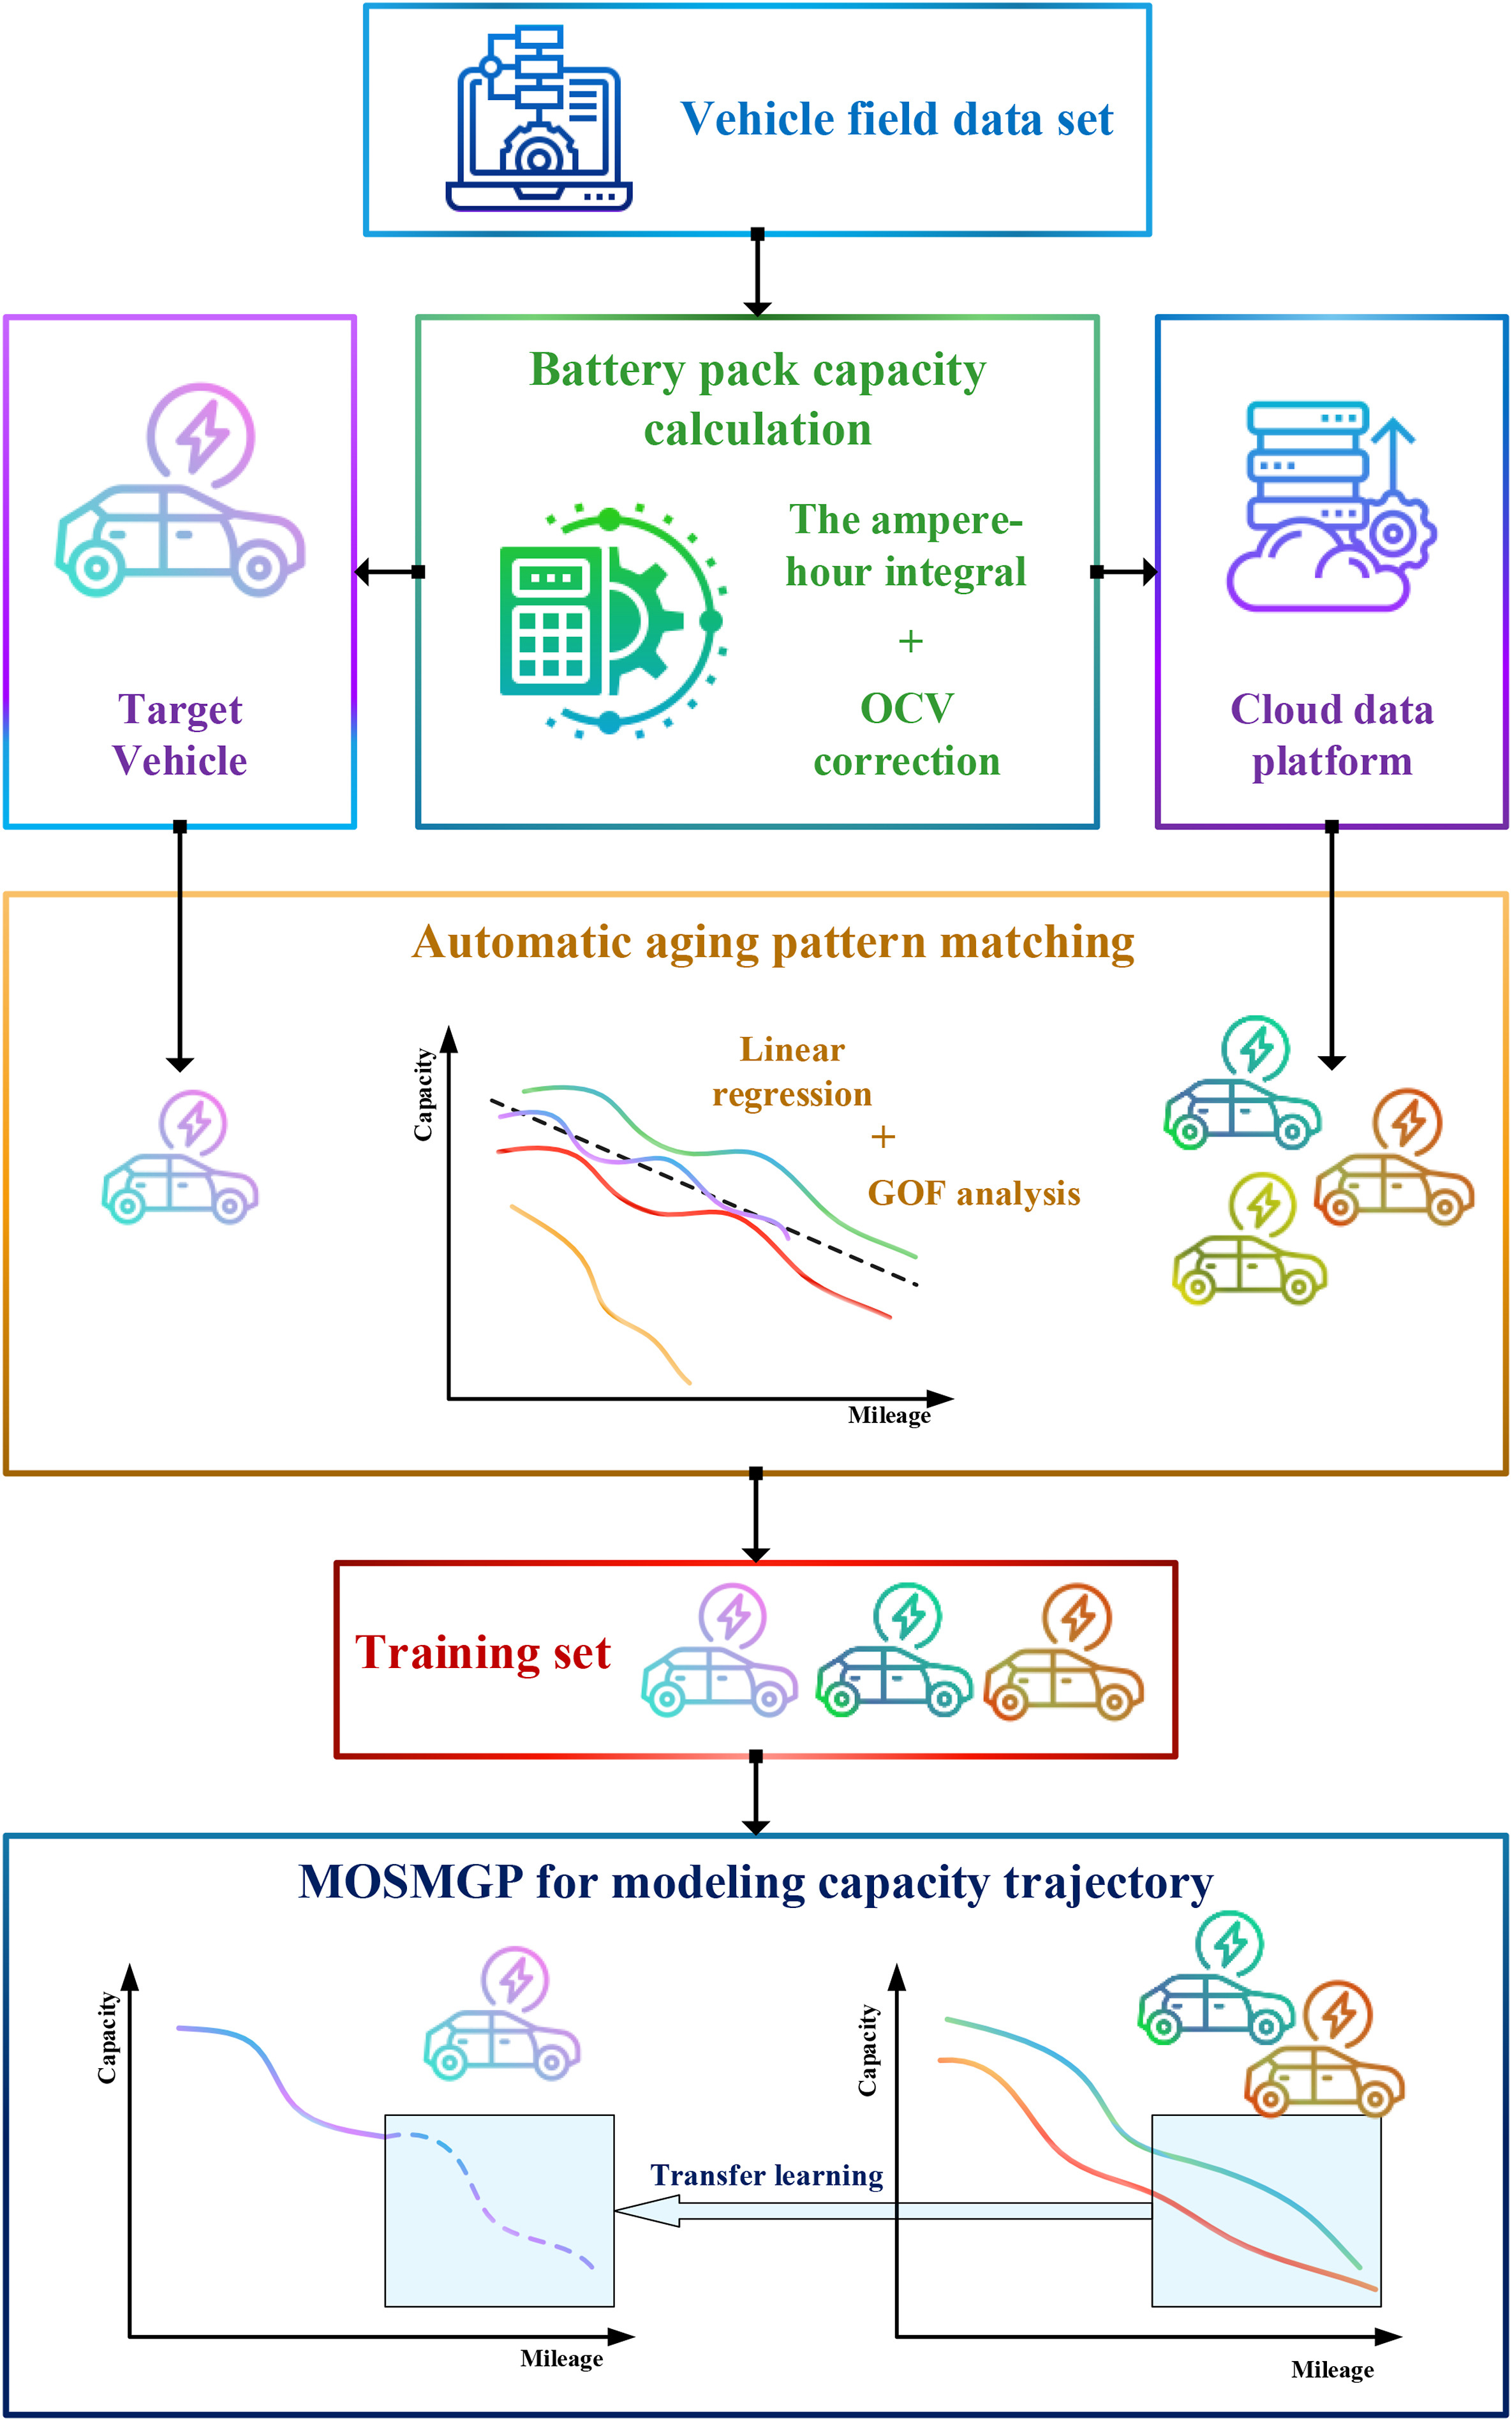
\includegraphics[height=1.0\linewidth]{resources/images/nn-vehicle-fleet-data}
	\caption{Ansatz zur zukünftigen \acs{SoH}-Bestimmung von Flottenfahrzeugen \cite{nnVehicleFleetData}}
	\label{fig:nn-vehicle-fleet-data}
\end{figure}